\documentclass[a4paper,11pt]{article}

\usepackage{times}
%\setcounter{secnumdepth}{0} % sections are not getting numbered
\usepackage[english,serbian]{babel}


\usepackage[T1]{fontenc} 
\usepackage{biblatex} % bibliography

\addbibresource{citation.bib} % file with references


\usepackage{comment}
\usepackage{amsfonts}
\usepackage{amsmath}
\usepackage{amsthm}
\usepackage{IEEEtrantools}
\usepackage{graphicx}
%\usepackage{cite}

%\usepackage{geometry}
%\usepackage{upgreek}
\usepackage[serbian]{babel}
%\usepackage{ulem}
%\usepackage{environ}
\usepackage{tikz}
\usepackage{color}
\usepackage{fancybox}

%\numberwithin{equation}{section}
\theoremstyle{definition} \newtheorem{deff}{Definicija}[section]
\theoremstyle{definition} \newtheorem{prim}[deff]{Primer}
\theoremstyle{plain} \newtheorem{teor}[deff]{Teorema}


\newcommand{\unija}[2]{#1 \cup #2}
\newcommand{\pres}[2]{#1 \cap #2}
\newcommand{\tnorm}{$t$-norm}
\newcommand{\tkonorm}{$t$-konorm}


\renewenvironment{proof}[1][\proofname]{{\bfseries #1.}}

\frenchspacing


\usepackage[a4paper,top=3cm,bottom=2cm,left=2cm,right=2cm,marginparwidth=1.75cm]{geometry}
%% Useful packages
\usepackage{mathrsfs}
\newsavebox\foobox
\newlength{\foodim}
\newcommand{\slantbox}[2][0]{\mbox{%
		\sbox{\foobox}{#2}%
		\foodim=#1\wd\foobox
		\hskip \wd\foobox
		\hskip -0.5\foodim
		\pdfsave
		\pdfsetmatrix{1 0 #1 1}%
		\llap{\usebox{\foobox}}%
		\pdfrestore
		\hskip 0.5\foodim
}}
\def\Laplace{\slantbox[-.45]{$\mathscr{L}$}}

%\usepackage[colorinlistoftodos]{todonotes}

\usepackage{caption}
\usepackage{subcaption}
\usepackage{changepage}


\usepackage{blindtext}

\usepackage{tabularx}
\usepackage[export]{adjustbox}

\usepackage[utf8]{inputenc}
\usepackage[T1]{fontenc}
\usepackage{lmodern}
\usepackage{graphicx}
\usepackage{color}
\usepackage{listings}
\usepackage{amsmath}

%\usepackage[usenames,dvipsnames]{xcolor}
%\usepackage[colorlinks=true,linkcolor=blue]{hyperref}

\usepackage{amsfonts}
\usepackage{epstopdf}

\usepackage{float}

\usepackage[shortlabels]{enumitem}
\usepackage[yyyymmdd]{datetime}


\renewcommand{\figurename}{Slika}

\DeclareMathOperator*{\argmax}{\arg\max}
\graphicspath{{./images/}}

\usepackage{booktabs}

\usepackage{siunitx}

\usepackage{scalerel}




\sloppy

\epstopdfsetup{update} % only regenerate pdf files when eps file is newer

%%%%%%%% DOCUMENT %%%%%%%%
\setlength {\marginparwidth }{2cm}
\begin{document}
	
	%%%% Title Page
	\begin{titlepage}
		
		\newcommand{\HRule}{\rule{\linewidth}{0.5mm}} 							% horizontal line and its thickness
		\center 
		
		% University
		\textsc{\LARGE Elektrotehnički fakultet u Beogradu}\\[1cm]
		
		% Document info
		\textsc{\Large Optimalno upravljanje sistemima}\\[0.2cm]
		\textsc{\large 13M051OUS}\\[1cm] 										
		\HRule \\[0.8cm]
		{ \huge \bfseries Upravljanje dvostrukim inverznim klatnom}\\[0.7cm]								% Assignment
		%\HRule \\[2cm]
		\textsc{\large Projektni zadatak broj 2}\\[1cm]
		
		
		\large
		\vfill 
		\emph{Studenti:}\\
		Nikita Jokić 3279/2023\\[0.1cm]
		Ivona Dučić 3067/2023\\[1.5cm]		
		\emph{Mentor:}\\
		doc. dr Aleksandra Krstić\\[0.1cm]									
		{\large Februar 2024}\\[2cm]
	\end{titlepage}
	\tableofcontents
	\newpage
	
	\section{Modeliranje sistema i analiza modela}
	\subsection{Uvod} 
	
	Furuta penduluma (FP) je rotaciono klatno koje se pokreće motorom jednosmerne struje. Dva najveća zahteva u vezi sa ovim sistemom su podizanje klatna iz donjeg u gornji položaj i održavanje klatna u uspravnom, nestabilnom ravnotežnom stanju. U ovom radu razmatrane su kontrolne strategije za nelinearni problem uspravljanja i balansiranja FP u uspravnom  položaju. Iako ovo može delovati kao akademski problem, FP je ilustrativan za širok spektar dinamičkih sistema sa stvarnim primenama. Fokusiranje na ovu problematiku integrisano je u aktuelna istraživanja u oblasti sajber-fizičkih sistema (CPSs)\footnote{Sajber-fizički sistemi (CPSs) predstavljaju integraciju računarskih elemenata sa fizičkim sistemima, stvarajući tako dinamičko i uzajamno povezano okruženje.} \cite{inicijalna}. \\ 
	
	%	Fizičari su uspešni u modelovanju fenomena u prirodi u iznenađujućem broju redova veličina. Iako se u većini slučajeva može samo težiti posmatranju, u malom, ali važnom podskupu, moguće je aktivno modifikovati ponašanje sistema. Ovo se postiže uključivanjem računarskih komponenti koje interaguju sa fizičkim sistemom, što čini osnovu istraživanja u oblasti sajber-fizičkih sistema. Teorija upravljanja se bavi izazovima u postizanju željenih performansi sistema, uključujući nestabilnost u otvorenoj sprezi, ograničenja u broju promenljivih koje se mogu aktivirati i ograničene informacije o stanju sistema.\\
	
	%	Ovaj rad proučava sisteme koji se mogu modelovati konačnim brojem povezanih diferencijalnih jednačina prvog reda, kako linearne sisteme tako i nelinearne sistema, koji su prisutni u sve većem broju modernih aplikacija. \\
	
	Furuta pendulum, kao jednostavan primer nelinearnog sistema, služi kao osnovno sredstvo za istraživanje ideja u oblasti nelinearnog upravljanja. Takođe predstavlja prototip za praktično važne uređaje poput robotskih ruku cilindričnog oblika, rotacionih dizalica ili transportnih sistema za visoke objekte. Kontrolni problemi usmeravanja i balansiranja penduluma oko nestabilne ravnoteže su dobro proučeni.\\
	
	U rada \cite{inicijalna} se navodi da do trenutka kada je rad napisan, nelinearni problem uspravljanja FP nije rešavan optimalnom kontrolom. Korišćenjem optimalne kontrole, problem se elegantno formuliše kao minimizacija odgovarajućeg troška uz poštovanje određenih ograničenja. Primenom ove tehnike, autor istražuje savremene tehnike kontrole, njihovu primenljivost u sličnim problemima i razvija odgovarajuću kontrolnu tehniku za ovu klasu uređaja. Pored optimalne kontrole uspravljanja FP razmatrane su i ad hoc strategije koje se oslanjaju na zakone upravljanja izvedene iz analize sistema. Balansiranje klatna oko njegovog nestabilnog ravnotežnog stanja se obavlja korišćenjem LQG. 
	
	(uvod doraditi na kraju, navesti strukturu izvestaja...) napisati da je prvi deo nelinerno upravljanje, a balansiranje lineran...za prebacijvanje kontroler.. sistem nestabilan u otvorenoj sprezi, vodi se racuna da  pri prebacivanju ne dodje do nestabilnost, koriscenje linearnog, nelinearnog modela..
	
	\newpage
	
	\subsection{Modeliranje sistema} 
	
	Modeli su ključni elementi u projektovanju kontrolera jer omogućavaju simulaciju sistema i testiranje kontrolera u preliminarnoj fazi, u offline režimu. U slučaju korišćenja nelinearnih MPC kontrolera, zahteva se da model bude ugradjen u sistem.  \\
	
	U zavisnosti od pristupa koji se koristi, za dizajn kontrolera potrebni su različiti tipovi modela. Pristupi koji se primenjuju za podizanje klatna iz donjeg u gornji položaj, kao što su ad hoc i optimalno upravljanje zahtevaju nelinearne modele, jer sistem prati putanju u prostoru stanja koja prolazi kroz različite regione sa različitom dinamikom. S druge strane, održavanje klatna u gornjem položaju zahteva samo kontroler koji može raditi u lokalnom regionu, te je za postizanje ovog cilja potreban samo linearni model.  \\
	
	Linearni modeli su mogu dobiti na dva načina: Jakonijan linearnizacijom nelinearnog modela u okolini želeljenog ravnotežnog stanja ili tehnikama identifikacije, gde se parametri linearnog modela procenjuju iz ekseprimenata. U otvorenoj sprezi, gornji položaj je nestabilan, i ako se primeni mala smetnja na ulazu, izlazni signal će rasti bez ograničenja. Da bi se izbegao ovaj problem, potrebno je prikupiti podatke u slučaju kada se na sistem primeni upravljanje sa stabilnim kontrolerom.  Oblast identifikacije je detaljno proučavana krajem 1960-ih i početkom 1970-ih  \cite{identifikacija}. Glavni izazov je bio kako ukloniti šum koji se kontaminira sa ulazom i izlazom sistema.  \\
	
	
	Furuta pendulum je dinamički sistem koji se sastoji od dve osnovne komponente: \\
	
	Horizontalna ruka: Ovo je čvrsta šipka ili krak koji je postavljen horizontalno. Na jednom kraju može biti pričvršćen za oslonac, dok je drugi kraj često povezan sa vertikalnim delom sistema, poznatim kao pendulum. Horizontalna ruka služi kao platforma za postavljanje i rotiranje vertikalnog penduluma. \\
	
	Vertikalni pendulum: Ovaj deo predstavlja masu (obično šipka ili krak) koje je povezano sa horizontalnom rukom na jednom kraju, a drugi kraj se slobodno kreće. Rotacija penduluma oko vertikalne ose može se kontrolisati pomoću motora koji je integrisan u sistem. Ovaj motor omogućava sistemu da realizuje oscilatorne pokrete.\\
	
	\begin{figure}[!htb]
		\centering
		\begin{subfigure}{0.3\linewidth}
			\centering
			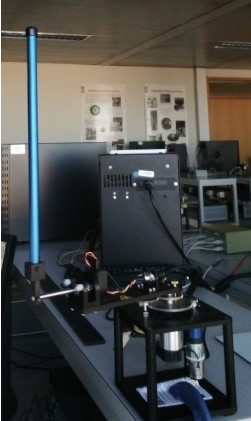
\includegraphics[width=\linewidth]{slike/eksperiment.jpg}
			\caption{}
			\label{fig:eksper}
		\end{subfigure}
		\hfill
		\begin{subfigure}{0.5\linewidth}
			\centering
			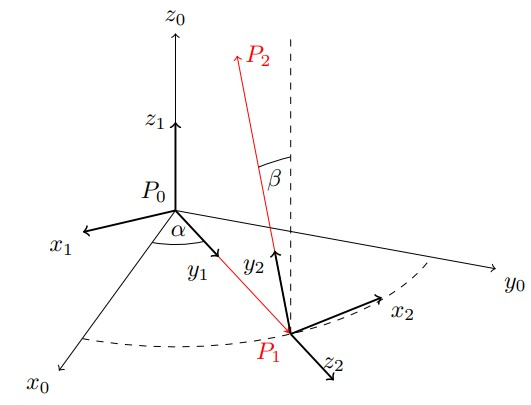
\includegraphics[width=\linewidth]{slike/shema.jpg}
			\caption{}
			\label{fig:schema}
		\end{subfigure}
		\caption{(a) Aparatura za ekepriment, (b) šematski prikaz inverznog klatna \cite{inicijalna} }
	\end{figure}
	
	
	Na slici (\ref{fig:schema}) prikazan je šematski prikaz inverznog klatna. Horizontalna ruka je predstavljena segmentom $P_0$ i $P_1$, dok je klatno predstavljeno segmentom $P_1$ i $P_2$, ugao $\alpha$ predstavlja zglob izmedju baze i horizontalne ruke FP, dok $\beta$ predstavlja ugao izmedju horizontalne ruke i klatna.
	\\
	
	Nelinearni model FP izveden je iz Langranžove mehanike. Energija sistema koji se sastoji od N krutih tela može se napisati kao zbir kinetičke energije $\tau$ i potencijalne energije $\nu$ \cite{inicijalna}. 
	\begin{equation}
		\tau = \sum_{i=1}^{N} \left( \frac{1}{2} M_i |v_i|^2 + \frac{1}{2} \omega_i I_i \omega_i^T \right)
	\end{equation}
	
	\begin{equation}
		\nu = \sum_{i=1}^{N} M_i \cdot (-g)
	\end{equation}
	
	
	
	Gde za svako kruto telo $i$, $M_i$ je masa tela, $v_i$ je brzina centra mase, $I_i$ matrica inercije, $\omega_i$ ugaona brzina, $r_i$ pozicija od centra mase, i $g$ je gravitaciono ubrzanje.\\
	
	Langranžijan se računa kao :
	
	\begin{equation}
		\mathcal{L} = \tau - \nu, 
	\end{equation}
	
	dok se jednačine kretanja računaju preko Ojler-Langranžovih jednačina: 
	\begin{equation}
		\frac{d}{dt} \left(\frac{\partial \mathcal{L}}{\partial \dot\alpha}\right) - \frac{\partial \mathcal{L}}{\partial \alpha} = -K_{a_1} \dot\alpha + K_f i, \quad 
	\end{equation}
	
	\begin{equation}
		\frac{d}{dt} \left( \frac{\partial \mathcal{L}}{\partial \dot\beta} \right) - \frac{\partial \mathcal{L}}{\partial \beta} = -K_{a_2} \dot\beta
	\end{equation}
	
	Karakteristika motora data je jednačinom: 
	\begin{equation}
		\frac{d}{dt} \left( L_b \frac{di}{dt} \right) + K_t \frac{d\alpha}{dt} + R i = u
	\end{equation}
	
	Kako bi se konstruisao nelinearni model sistema u prostoru stanja: 
	\begin{equation}
		\dot x = f(x, u)
	\end{equation}
	promenljive se definišu kao: $x_1$ = $\alpha$, $x_2$ = $\dot\alpha$,  $x_3$ = $\beta$, $x_4$ = $\dot\beta$, $x_5$ = $i$. \\
	
	
	Pri modelovanju i odredjivanju parametara sistema
	zanemarene su dinamičke karakteristike sistema: ne-elektične disipativne sile modelovane su kao viskozno trenje proporcionalnoj ugaonoj brzini zglobova, spoj između tela smatra se savršenim, uticaj, promena električnih karakteristika usled promene temperature aktuatora, zanemarivanje kapaciteta i induktivnosti žica raspodelejnih u prostoru i mehanički delovi su smatrani potpuno krutim.\\
	
	
	Konačno model u prostoru stanja glasi:
	
	\begin{equation}
		\begin{aligned}
			\dot{x}_1 &= x_2; \\[0.8em]
			\dot{x}_2 &= -\frac{J_2(K_{a1}x_2 - K_fx_5 + x_4(L_{cm2}L_{e1}m_2x_4 + 2J_2x_2\cos(x_3))\sin(x_3))}{-L_{cm2}^2L_{e1}^2m_2^2\cos(x_3)^2 + J_2(J_0 + J_2\sin(x_3)^2)} \\[0.8em]
			&\quad + \frac{L_{cm2}L_{e1}m_2\cos(x_3)(-K_{a2}x_4 + (gL_{cm2}m_2 + J_2x_2^2\cos(x_3))\sin(x_3))}{-L_{cm2}^2L_{e1}^2m_2^2\cos(x_3)^2 + J_2(J_0 + J_2\sin(x_3)^2)}; \\[0.8em]
			\dot{x}_3 &= x_4; \\[0.5em]
			\dot{x}_4 &= \frac{K_{a2}x_4 - gL_{cm2}m_2\sin(x_3)(J_0 + J_2\sin(x_3)^2)}{L_{cm2}^2L_{e1}^2m_2^2\cos(x_3)^2 - J_2(J_0 + J_2\sin(x_3)^2)} \\[0.8em]
			&\quad + \frac{\cos(x_3)(-J_0J_2x_2^2 + L_{cm2}^2L_{e1}^2m_2^2x_4^2)\sin(x_3)}{L_{cm2}^2L_{e1}^2m_2^2\cos(x_3)^2 - J_2(J_0 + J_2\sin(x_3)^2)} \\[0.8em]
			&\quad - \frac{J_2^2x_2^2\sin(x_3)^3 + L_{cm2}L_{e1}m_2(K_{a1}x_2 - K_fx_5 + J_2x_2x_4\sin(2x_3))}{L_{cm2}^2L_{e1}^2m_2^2\cos(x_3)^2 - J_2(J_0 + J_2\sin(x_3)^2)};\\[0.5em]
			\dot{x}_5 &= -\frac{K_tx_2 - Rx_5 + u}{L_b}.
		\end{aligned}
		\label{eq:nonModel}
	\end{equation}\\
	
	U radu \cite{inicijalna} za identifikaciju parametara korišćena je metoda najmanjih kvadrata (mozda dopisati jos koju recenicu). Eksperiment su izvodili nad aparaturom prikazanom na slici (Sl. \ref{fig:eksper}). Rezultati su predstavljeni u tabeli \ref{tab:tab1}.
	
	\begin{table}[ht]
		\centering
		\caption{Vrednosti i opis parametara sistema}
		\begin{tabular}{l l l l}
			\toprule
			Parametar & Vrednost & Jedinica & Opis promenljive \\
			\midrule
			$L_{e1}$ & $227 \pm 1$ & mm & Dužina horizontalne ruke, FP \\
			$J_0$ & $86.98 \pm 0.03$ & g $\cdot$ m$^2$ & Moment inercije na spoju baze horizontalne ruke i klatna, FP \\
			$K_{a1}$ & $1.0 \pm 0.3$ & mN $\cdot$ m $\cdot$ s & Koeficijent trenja između baze i horizontalne ruke, FP \\
			$M_2$ & $309 \pm 1$ & g & Masa klatna, FP \\
			$L_{cm2}$ & $404 \pm 1$ & mm & Udaljenost od ose rotacije do centra mase klatna, FP \\
			$J_2$ & $28.37 \pm 0.01$ & g $\cdot$ m$^2$ & Moment inercije na spoju klatna, FP \\
			$K_{a2}$ & $0.136 \pm 0.001$ & mN $\cdot$ m $\cdot$ s & Koeficijent trenja između horizontalne ruke i klatna, FP \\
			$L_b$ & $3.0 \pm 0.1$ & mH & Električna impedansa motora (imaginarni deo), FP \\
			$R$ & $2.266 \pm 0.002$ & $\Omega$ & Električni unutrašnji otpor motora, FP \\
			$K_t$ & $0.696 \pm 0.001$ & V $\cdot$ s & Kontra-elektromotorne sile, FP \\
			$K_f$ & $3.377 \pm 0.002$ & V & Obrtni moment koji proizvodi motor po jedinici struje, FP \\
			\bottomrule
		\end{tabular}
		\label{tab:tab1}
	\end{table}
	
	
	
	
	\subsubsection{Matlab model}
	
	
	
	
	
	
	\clearpage
	
	
	\subsection{Ponašanje sistema u otvorenoj sprezi}
	
	
	
	\clearpage 
	\subsection{Linearizacija sistema}
	\label{sec:linearizacija}
	
	Nelinearni model (\ref{eq:nonModel}) se može linearizovati razvijanjem u Tejlorov red u okoline tačke $(\bar{x}, \bar{u})$:
	\begin{equation}
		\mathbf{f}(\mathbf{x}, u) \approx \mathbf{f}(\mathbf{\bar{x}}, \bar{u}) + \nabla_x \mathbf{f}|_{(\bar{x},\bar{u})} (\mathbf{x} - \mathbf{\bar{x}}) + \frac{\partial \mathbf{f}}{\partial u}|_{(\mathbf{\bar{x}},\bar{u})} (u - \bar{u}). \label{eq:linearization}
	\end{equation}
	
	Neka su $A = \nabla_{\mathbf{x}} \mathbf{f}|_{(\bar{\mathbf{x}},\bar{u})}$, $B = \frac{\partial \mathbf{f}}{\partial u}|_{(\bar{\mathbf{x}},\bar{u})}$, $\Delta \mathbf{x} = \mathbf{x} - \bar{\mathbf{x}}$, i $\Delta u = u - \bar{u}$.
	Prethodna jednačina se može napisati kao:
	\begin{equation}
		\dot{\mathbf{x}} \approx A\Delta \mathbf{x} + B\Delta u + f(\bar{\mathbf{x}}, \bar{u}). \label{eq:linearized_system}
	\end{equation}
	
	Linearizacija se obavlja za različite $\bar{\mathbf{x}}$ čime se dolazi do porodice linearnih modela. Linearni model u okolini tačke  $f(\bar{x} = 0, u = 0) = 0$, može se napisati kao:
	\begin{align}
		\begin{split}
			\dot{x}(t) &= Ax(t) + Bu(t) \\
			y(t) &= Cx(t) + Du(t)
		\end{split}
		\label{eg:lin_mod}
	\end{align}
	
	
	gde  $x$, $u$, i $y$ označavaju odstupanje od ravnotežnog stanja
	\[
	\mathbf{A} =
	\begin{bmatrix}
		0 & 1.0000 & 0 & 0 & 0 \\
		0 & -0.0174 & 20.7861 & -0.0023 & 57.5344 \\
		0 & 0 & 0 & 1.0000 & 0 \\
		0 & -0.0174 & 63.8319 & -0.0071 & 57.4388 \\
		0 & -232.0252 & 0 & 0 & -755.4250
	\end{bmatrix}
	\]
	
	\[
	\mathbf{B} =
	\begin{bmatrix}
		0 \\
		0 \\
		0 \\
		0 \\
		333.3367
	\end{bmatrix}
	\]
	
	\[
	\mathbf{C} =
	\begin{bmatrix}
		1 & 0 & 0 & 0 & 0 \\
		0 & 0 & 1 & 0 & 0
	\end{bmatrix}
	\]
	
	\[
	\mathbf{D} =
	\begin{bmatrix}
		0 \\
		0
	\end{bmatrix}
	\]
	
	
	\subsubsection{Kontrolabilnost}
	
	Kontinualni linearni sistem se smatra potpuno kontrolabilnim ako i samo ako iz početnog stanja, uz odgovarajući ulaz $u(t)$ sa $0 < t \leq t_f$ i konačnim horizontom $t_f$, može da se postigne
	proizvoljno stanje $x(t_f) = x_f$. \\
	
	Linearni sistem je potpuno kontrolabilan ako matrica kontrolabilnosti
	\begin{align}
		C[A, B] = \begin{bmatrix}
			B & AB & A^2B & \cdots & A^{n-1}B
		\end{bmatrix} 
	\end{align}
	
	ima pun rang $n$. \\
	
	Kada se napon primeni na motor, stvara se struja i obrtni moment $\tau_1$ se stvara u centru rotacije horizontalne ruke. Na metalnom vratilu gde je klatno pričvršćeno, sila nastala od $\tau_1$ duž ruke $l_{e1}$ je horizontalna i pravolinijska u odnosu na oba $l_{e1}$ i $\tau_1$, u skladu sa opštom formulom
	
	\begin{align}
		\tau = r \times F. \quad 
	\end{align}
	
	Obrtni moment u centru mase klatna takođe je dat ovom formulom, iz kojeg se može izraziti amplituda $\tau_2$ kao funkcija ugla $\beta$
	
	\begin{align}
		\tau_2 = l_{cm2} F \cos \beta, \quad
	\end{align}
	
	
	gde je $l_{cm2}$ rastojanje između metalnog vratila i centra mase klatna. Iz gornjih jednačina jasno je da je ulaz, napon primenjen na motor, direktna akcija na sve stanja sistema - struju motora, položaj i brzinu horizontalne ruke, kao i položaj i brzinu klatna. Postoji izuzetak za $\cos \beta = 0$, tj. kada je klatno horizontalno. U ovom slučaju, položaj i vektorske sile su paralelni, te stoga nije moguće primeniti obrtni moment. Stoga, varijable klatna nisu kontrolabilne u ovom trenutku.
	
	
	\subsubsection{Opservabilnost}
	
	Kontinualni sistem se smatra potpuno opservabilnim ako je poznavanje $y(t)$ za $0 \leq t \leq t_1$, sa $t_1$ konačnim, dovoljno za određivanje početnog stanja $x(0)$. \\
	
	Linearni sistem je opservabilan ako matrica
	
	\begin{align}
		O(A, C) = \begin{bmatrix}
			C \\
			CA \\
			CA^2 \\
			\vdots \\
			CA^{n-1}
		\end{bmatrix} \quad
	\end{align}
	ima pun rang $n$.
	
	\subsubsection{Stabilnost}
	
	
	
	Tačka \(\bar{x}\) dinamičkog sistema se klasifikuje kao Liapunov stabilna ako važi:
	\begin{align}
		\forall \epsilon > 0, \exists \delta > 0 : ||x(0) - \bar{x}|| < \delta \land t > 0 \Rightarrow ||x(t) - \bar{x}|| < \epsilon, \quad 
	\end{align}
	i asimptotski stabilna ako dodatno važi:
	
	\begin{align}
		\exists \epsilon > 0 : ||x(0) - \bar{x}|| < \epsilon \Rightarrow \lim_{t \to \infty} x(t) = \bar{x}. \quad
	\end{align}
	
	Asimptotska stabilnost nelinearnog sistema može se proceniti linearnizovanim sistemima dobijenim kod svake fiksne tačke pomoću Liapunovljeve indirektne metode. Moguće je zaključiti da, za linearnizovani sistem (\ref{eg:lin_mod}):
	\begin{enumerate}
		\item ako sve sopstvene vrednosti matrice \(A\) imaju negativne realne delove, tada je fiksna tačka nelinearnog sistema stabilna;
		\item ako bar jedna sopstvena vrednost matrice \(A\) ima pozitivan realni deo, tada je fiksna tačka nelinearnog sistema nestabilna;
		\item ako nijedno od prethodno navedenog nije zadovoljeno, tj. ako bar jedna sopstvena vrednost leži iznad imaginarne ose, a nema sopstvene vrednosti sa pozitivnim realnim delom, onda se ne može izvesti zaključak.
	\end{enumerate} 
	
	
	
	\begin{table}[H]
		\centering
		\caption{Sopstvene vrednosti linearizovanih modela, asimptotska stabilnost redukovanog sistema ($X_2, \cdots, X_5$), kontrolabilnost i observabilnost za 5 tačaka, gde su sve promenljive stanja postavljene na nulu, osim $X_3$.}
		\label{table:eigenvalues}
		\begin{tabular}{c c c c c c c}
			\hline
			$X_3$ & Sopstvene vrednosti & Stabilan & Kontrolabilan & Observabilan \\
			\hline
			0 & $-737.2$, $-19.4$, $+7.0$, $-5.8$, $0$ & Ne & Da & Da \\
			$\pi/4$ & $-743.2$, $-11.8$, $-5.3$, $+5.0$, $0$ & -- & Da & Da \\
			$\pi/2$ & $-746.2$, $-9.1$, $-0.0$, $0$, $0$ & -- & Ne & Da \\
			$3\pi/4$ & $-743.2$, $-12.4$, $+0.1 + 5.0i$, $+0.1 - 5.0i$, $0$ & -- & Da & Da \\
			$\pi$ & $-737.2$, $-17.0$, $-0.5 + 6.8i$, $-0.5 - 6.8i$, $0$ & Da & Da & Da \\
			\hline
		\end{tabular}
		\label{tab:5_tacaka}
	\end{table}
	
	U tabeli \ref{tab:5_tacaka} je prikazana analiza za 5 različitih tačaka, čime se pokazuje da je $x_3 = 0$ (kada se sistem se nalazi u gornjem položaju) nestabilno stanje, ali ispunjave uslove kontrolabilnosti i opservabilnosti.
	
	\clearpage
	\subsection{Poremećaji u sistemu}
	
	
	
	
	\clearpage
	\subsection{Upravljački signali i skaliranje signala}
	
	
	
	
	\newpage
	
	
	
	\section{Projektovanje sistema upravljanja}
	
	Projektovanje sistema upravaljanja se sastoji iz dva dela: generisanje željene trajektorije i projektovanje kontrolera koji treba da isprati željenu trajektoriju i održava sistem u gornjem položaju. \\
	
	Često je korisno dizajnirati putanje van mreže, tj. definisati putanju u prostoru stanja koju sistem treba da izvede unapred. U takvoj situaciji nismo ograničeni vremenom ili računski potrebnom snagom da se izvrše proračuni tokom samog procesa, što je posebno korisno kod složenih sistema sa brzom dinamikom. Putanje se dizajniraju koristeći model sistema, analizirajući njegov odgovor na dostupne ulaze. Ova strategija se široko koristi u robotici, gde postoji potreba za planiranjem kretanja mobilnih robota u ograničenim prostorima \cite{inicijalna}. \\
	
	Jedan od pristupa za generisanje trajektorije je optimalno upravljanje,  koje se bavi problemom određivanja ulaza dinamičkog sistema koji opitmizuje (maksimizuje ili minimizuje) odredjenu funkciju troška koja govori o performansama sistema. Sa odgovrajućom funkcijom troška mogu se odrediti putanja i zakon upravljanja koji zadovoljava zahteve projektovanja. Takodje, većina nelinearnih problema se može rešiti oslanjanjem na numeričke metode. \\
	
	Nakon što se izgeneriše trajektorija, potrebno je isprojektovati kontroler koji će pratiti zadati putanju. U radu \cite{inicijalna} su predložena ...
	
	
	
	
	\newpage
	\subsection{Generisanje trajektorije}
	
	Ovo poglavlje istražuje kako pronaći optimalan ulaz za dinamički sistem, omogućavajući mu da sledi željenu putanju u prostoru stanja. Ova putanja treba da bude u skladu sa zadanim ograničenjima i optimizuje zadatu veličinu. Iako se različite strategije mogu koristiti za projektovanje putanja, fokus je stavljen na optimalno upravljanje. Ova tehnika pruža jasan okvir za pronalaženje rešenja za probleme podložne ograničenjima i ciljevima optimizacije. Pored optimalnog generisanja trajektorije, implementirane su i ad hoc metode za uspravljanje klatna kao alternativno i jednostavno rešenje. 
	
	\subsubsection{Ad hoc strategije}
	\label{sec:andhoc}
	
	Jedna od najčešće korišćenih metoda za podizanje FP je kontrola energije. U ovom slučaju se energija sistema kontroliše umesto direktnog kontrolisanja pozicije i brzina klatna \cite{inicijalna}.
	U \cite{energy_c} predložen je zakon upravljanja za uspravljanje klatna zasnovanoj na kontroli energije (engl: Energy control): \\
	
	\begin{equation}
		u = \text{\textit{sat}}\left[k_v (E - E_0)\right] \text{\textit{sign}}( \dot{\beta} \cos \beta), 
		\label{eq:en_control}
	\end{equation} \\
	
	
	gde su $\textit{E}$ trenutna energija sistema, 
	$\textit{E}_0$ je željena energija sistema, $\textit{k}_v$ je pojačanje kontrolera, a $\beta$ je ugao penduluma. Prvi pojam definiše amplitudu ulaza. Može se posmatrati kao proporcionalni kontroler, gde je promenljiva razlika u energiji između trenutnog stanja i energije ciljnog stanja, koja je konvencionalno postavljena na nulu. Amplituda je ograničena zbog fizičkih ograničenja aktuatora. Drugi pojam definiše znak upravljačkog ulaza i obezbeđuje da je efekat ulaza dodavanje energije sistemu. Član $\cos \beta$ procenjuje da li je trenutni položaj penduluma iznad ili ispod horizontalnog položaja. Za $\cos \beta = 0$, pendulum je horizontalan, stoga sistem nije kontrolabilan - nema prenosa energije na pendulum. Sa dodatnim članom $\dot{\beta}$, sila se primenjuje protiv smera kretanja penduluma kada je ispod horizontalnog položaja i u istom smeru kada je iznad.\\
	
	Važno je napomenuti da je ovaj zakon upravljanja projektovan specifično za sistem FP, stoga nije vrlo opšte primenljiv. Takođe, ograničen je na situacije gde nivo energije ciljnog stanja nije degenerisan. Iako će kontroler dovesti sistem do stanja sa određenom energijom, ako postoji više konfiguracija sa istom energijom, nije moguće izabrati između njih. Ovo je slučaj kod FP, gde energija sistema ne zavisi od ugla horizontalne ruke $\alpha$. Dakle, ovom tehnikom nema kontrole nad ovom varijablom tokom uspravljanja. \\
	
	Zakon upravljanja definisan u jednačini (\ref{eq:en_control}) zahteva izračunavanje energije sistema. Modifikovana verzija kontrolera predložena je u \cite{energy_c} koja uzima u obzir samo varijable prostora stanja. Ovaj zakon upravljanja poznate je kao 
	Exponentiation of the pendulum position i glasi:\\
	
	\begin{equation}
		u = \text{\textit{sat}}(k_v |\beta^n|) \text{\textit{sign}}( \dot{\beta} \cos \beta)
	\end{equation} \\
	
	U ovom slučaju, prvi član je modifikovan, sada uzimajući ugao između trenutnog položaja i vertikale.
	Dodaje se eksponent \textit{n} izražen u izrazu, što povećava amplitudu ulaza kada je pendulum daleko od uspravnog položaja, ali je manja kada je bliže. U \cite{inicijalna} navode da ovaj zakon omogućava glađi prelaz između nelinearnog upravljanja i upravljanja koji balansira klatno u gornjem položaju. Drugi član ostaje nepromenjen. \\
	
	U \cite{ener_shaping} je izveden i testiran zakon upravljanja poznat kao energy shaping. Pomenuti zakon upravljanja je izveden na osnovu inevrznog klatna koji rotira samo oko vertikalne ose i glasi: \\
	
	\begin{equation}
		u = k_1 (\dot\alpha + k_2 \cos(\beta) \dot\beta)	
	\end{equation}
	
	\subsubsection{Optimalno upravljanje}
	Optimalna kontrola se bavi problemom određivanja ulaza dinamičkog sistema koji optimizuju, tj. minimiziraju ili maksimiziraju, određeni indeks performansi. Sa odgovarajućim izborom funkcije troška, mogu se odrediti trajektorije i zakoni upravljanja tako da zadovolje zahteve dizajna.
	
	U ovom radu, koristili smo model prediktivnog upravljanja (engl. Model Predictive Control, MPC) kao pristup za optimalnu kontrolu. \\
	
	MPC koristi matematički model sistema kako bi predvidio buduće ponašanje sistema na osnovu trenutnog stanja i unapred zadatih referenci. Model može biti linearni ili nelinearni, ali je ključno da bude dovoljno tačan za predviđanje sistema u predvidjenom vremenskom horizontu. MPC optimizuje kontrolne akcije za određeni horizont vremena unapred. MPC ne razmatra samo trenutno stanje sistema, već razmatra niz budućih koraka, obično u diskretnim vremenskim koracima. Ovaj horizont može biti kratkoročan ili dugoročan, u zavisnosti od zahteva sistema i dinamike procesa. MPC minimizira ili maksimizira funkciju cilja koja predstavlja kriterijum performansi sistema. To može uključivati minimizaciju greške u praćenju referenci, minimizaciju potrošnje energije ili slične ciljeve. MPC primjenjuje samo prvu kontrolnu akciju iz optimizacionog problema, nakon čega se proces ponavlja u svakom diskretnom vremenskom koraku. Ovaj pristup omogućava MPC-u da reaguje na promjene u stanju sistema i spreči akumulaciju grešaka. Njegova sposobnost da predviđa buduće stanje sistema i optimizuje kontrolne akcije čini ga moćnim alatom za upravljanje sistemima sa kompleksnom dinamikom i nelinearnostima \cite{mpc}.\\
	
	
	\begin{figure}[!htb]
		\centering
		\begin{subfigure}{0.5\linewidth}
			\centering
			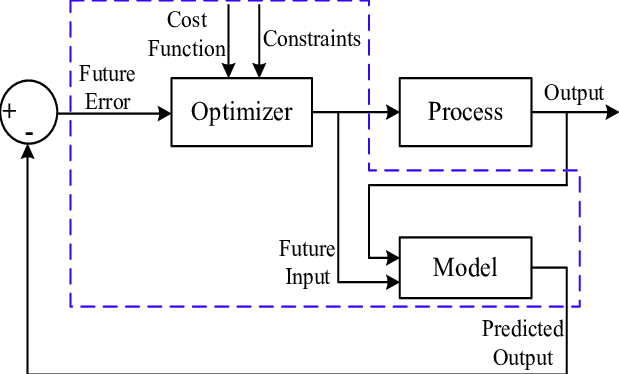
\includegraphics[width=\linewidth]{slike/mpc_sc.png}
			\caption{}
			\label{fig:mpc_sc}
		\end{subfigure}
		\hfill
		\begin{subfigure}{0.48\linewidth}
			\centering
			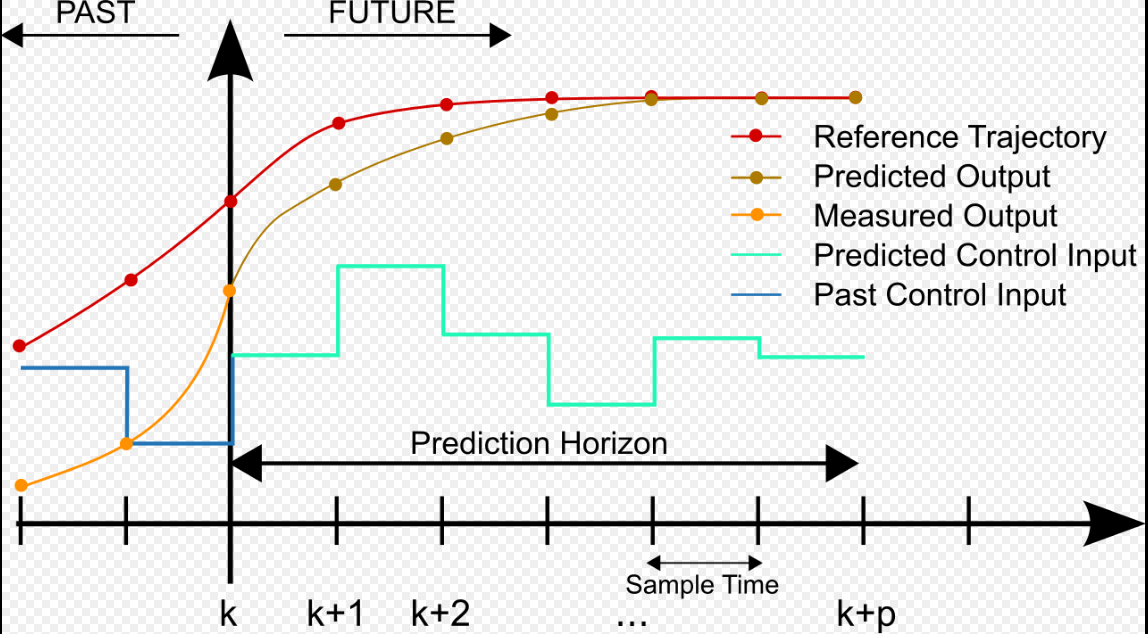
\includegraphics[width=\linewidth]{slike/mpc.png}
			\caption{}
			\label{fig:mpc_f}
		\end{subfigure}
		\caption{(a) Šema MPC-a, (b) ilustracija rada MPC-a \cite{mpc} }
	\end{figure}
	
	
	ovde treba doddati sta smo uzeli od parametra mpc, hotizont, funkije troska...imamo ih 2...CASADI?
	
	
	\newpage
	\subsection{Projektovanje kontrolera}
	
	Nakon generisanja referentnih trajektorije potrebno je projekotvati kontroler čiji je zadatak da u što većoj meri isprati željenu trajektoriju i kontroler koji će održavati sistem u željenom, gornjem položaja. \\
	
	Linearni kontroleri su validni samo u onom regionu gde je izvršena linearizacija sistema, a kako je zadatak upravlanje nelineranim sistemom potrebno je napraviti ansambl kontrolera. \\
	
	U radu \cite{inicijalna} su se bavili projektovanjem LQG kontrolera. Kalman filter je optimalan za procenu stanja u linearnim sistemima, ali kada se primeni na nelinearne sisteme, može doći do netačnih procena stanja zbog odstupanja između stvarne nelinearnosti sistema i linearnog modela koji se koristi u Kalman filtru. Iz ovog razloga, u ovom radu smo se zadržali na korišćenju LQR kontrolera. \\
	
	LQR (Linear Quadratic Regulator) je metoda optimalne kontrole koja se koristi za pronalaženje kontrolnih ulaza koji minimizuju određenu kvadratnu funkciju troška. LQR nudi nekoliko prednosti, uključujući jednostavnu implementaciju i robustnost, dok osigurava stabilnost sistema pod određenim uslovima. LQR kontroler ima nekoliko poželjnih svojstava, na primer, održava red sistema, ima faznu marginu od najmanje 60 stepeni i beskonačnu marginu pojačanja.\\
	
	Da bi se primenio LQR na sistem, dve osobine koje mora da zadovolji sistem je da bude kontrolabilan i opservabilan u okolini tačke gde je izvršena linearizacija sistema. Na osnovu analize prikazane u tabeli \ref{tab:5_tacaka} zaključuje se da jedino u slučaju kada je klatno u horizontalnom položaju ($\beta$ = $\pi /2$) nije moguće primeniti LQR kontroler.\\
	
	
	Cilj algoritma LQR je pronaći vektor pojačanja K za zakon povratne sprege u prostoru stanja
	\begin{equation}
		u = -Kx 
	\end{equation}
	
	koji se primenjuje na kontinualni linearni sistem, definisan u \ref{sec:linearizacija}, \\
	
	\begin{equation}
		\begin{cases}
			\dot{x}(t) = Ax(t) + Bu(t) \\
			y(t) = Cx(t) + Du(t)
		\end{cases}
	\end{equation}\\
	
	a minimizuje funkciju troška\\
	
	\begin{equation}
		J = \int_{0}^{\infty}  x^T Q_r x  + u^T R_r u
	\end{equation} \\
	
	Matrice $Q_r$ i $R_r$ određuju relativni značaj koji se pridaje regulaciji stanja i trošku ulaza, i treba ih odabrati uzimajući u obzir ciljeve dizajna sistema. Matrica $P$ se dobija rešavanjem Rikatijeve jednačine: \\
	\begin{equation}
		A^T P + P A - P B R^{-1} B^T P + Q_r = 0, 
	\end{equation} \\
	
	nakon čega se računa pojačanje $K$ kao:
	\begin{equation}
		K = R_r^{-1}BP, 
	\end{equation}
	
	\begin{figure}[!h]
		\centering
		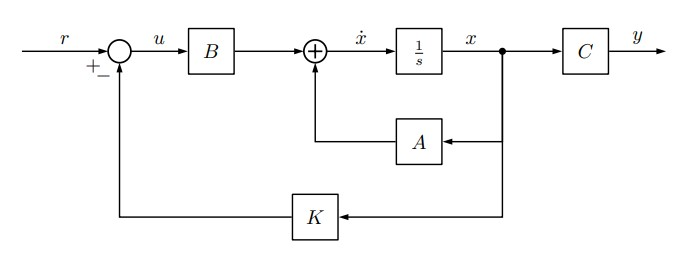
\includegraphics[width=0.8\linewidth]{slike/lqr.jpg}
		\caption{Blok dijagram feedback kontrolera \cite{inicijalna}}
		\label{fig:lqr}
	\end{figure}
	
	
	
	Prelazak između kontrolera vrši se u dva različita režima rada: \\
	
	1. Kontrola za podizanje sistema primenjuje se direktno na uređaj. Samo linearni kontroler oko krajnje tačke je aktivan (globalni LQR kontroler). Tranziciji između režima uspravljanja sistema i režima ravnoteže oko uspravnog poožaja se dešava kada se ugao penduluma dovoljno približi nultom položaju ($\beta$ < 18$^\circ$). Ovaj pristup se koristi kada nema referentne putanje, i podizanje sistema se izvodi u zatvorenoj petlji, na primer sa Ad hoc strategijama opisanim u \ref{sec:andhoc}. \\
	
	2. Referentna kontrola se primenjuje na uređaj, koji zauzvrat ima zatvoreni skup linearnih kontrolera koji stabilizuju razliku između izvedene putanje i referentne putanje. Ovo se naziva Gain Scheduling controller.\\
	
	Gain Scheduling kontroler implementiran u upravljanju FP bira jedan od šest kontrolera koji se koristi u skladu sa trenutnim uglom $\beta$. Važno je napomenuti da su oni raspoređeni simetrično: prvi član Tejlorovog reda je identičan za $\beta = \pm \theta$, pa je i inkrementalni model isti. 
	Na slici (Sl. \ref{fig:ganSc}) su prikazani regioni rada gain scheduling kontrolera, u funkciji ugla $\beta$ ($x_3$). Tačke označavaju mesta gde je izvedena Jakovijeva linearizacija, a $C_1$ do $C_6$ označavaju kontrolere koji rade u tom konkretnom regionu. Na primer $C_1$ radi za $\beta \in [-18^\circ, 18^\circ]$, i odgovoran je za održavanje klatna u uravnoteženom položaju na gore.
	
	\begin{figure}[!h]
		\centering
		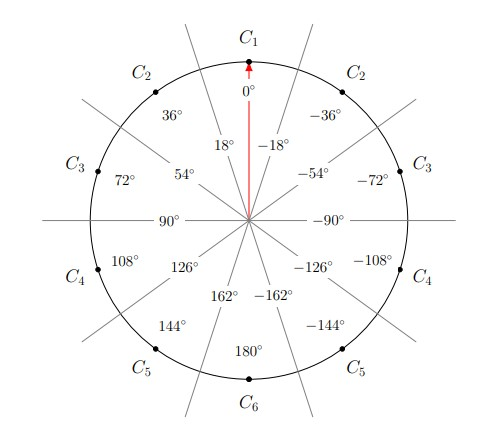
\includegraphics[width=0.6\linewidth]{slike/gainSc.jpg}
		\caption{Gain Scheduling kontroler \cite{inicijalna}}
		\label{fig:ganSc}
	\end{figure}
	
	Svaki LQR kontroler, koji je dizajniran nezavisno, koriguje vrednost ulazne promenljive kako bi aproksimirao ponašanje stvarnog sistema prema onom predviđenom u referentnoj putanji.
	
	\begin{figure}[!h]
		\centering
		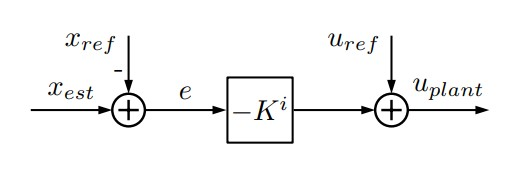
\includegraphics[width=0.5\linewidth]{slike/applyLqr.jpg}
		\caption{Arhitektura Gain Scheduling kontrolera. Vektor $K_i$, $i \in \{1, \ldots, 6\}$ se bira u skladu sa trenutnim uglom klatna \cite{inicijalna}}
		\label{fig:archGain}
	\end{figure}
	
	
	
	
	\newpage
	
	
	\section{Komparativna analiza projektovanih sistema upravljanja}
	
	\subsection{Poređenje odziva sistema}
	\subsubsection{Stabilizacija u gornjem položaju}
	
	\subsubsection{Robustnost na greške u modelovanju}
	\subsubsection{Uticaj šuma}
	
	\subsection{Potiskivanje poremećaja}
	
	
	
	
	\begin{table}[!h]
		\centering
		\begin{tabular}{|llllll|}
			\hline
			\multicolumn{6}{|c|}{Pore\dj{}enje kontrolera}                                                                                                                                                                                                                 \\ \hline
			\multicolumn{1}{|l|}{}              & \multicolumn{1}{l|}{slo"zenost} & \multicolumn{1}{l|}{pra\'cenje ref.} & \multicolumn{1}{l|}{potiskivanje porem.} &  \multicolumn{1}{l|}{multivarijabilnost} & prosek \\ \hline
			\multicolumn{1}{|l|}{$K_{dec}$}     & \multicolumn{1}{l|}{1}          & \multicolumn{1}{l|}{5}                              & \multicolumn{1}{l|}{3}                   &  \multicolumn{1}{l|}{5}    &  2.8   \\ \hline
			\multicolumn{1}{|l|}{$K_{dek0}$}    & \multicolumn{1}{l|}{2}          & \multicolumn{1}{l|}{4}                              & \multicolumn{1}{l|}{2}                   &  \multicolumn{1}{l|}{4}    & 2.4   \\ \hline
			\multicolumn{1}{|l|}{$K_{dek\omega_0}$} & \multicolumn{1}{l|}{3}          & \multicolumn{1}{l|}{3}                              & \multicolumn{1}{l|}{1}                   &  \multicolumn{1}{l|}{3}    & 2   \\ \hline
			\multicolumn{1}{|l|}{$K_{invF}$}  & \multicolumn{1}{l|}{4}          & \multicolumn{1}{l|}{2}                              & \multicolumn{1}{l|}{5}                   &  \multicolumn{1}{l|}{1}    & 2.4   \\ \hline
			\multicolumn{1}{|l|}{$K_{H_{\infty}}$}  & \multicolumn{1}{l|}{5}          & \multicolumn{1}{l|}{1}                              & \multicolumn{1}{l|}{4}                   &  \multicolumn{1}{l|}{2}    & 2.4   \\ \hline
			
		\end{tabular}
		\captionof{table}{}\label{poredjenje_kontrolera}
	\end{table}
	\vspace{1cm}
	
	
	\section{Zaklju"cak}
	
	
	\newpage
	
	\begin{thebibliography}{9}
		\bibitem{inicijalna}
		\emph{Nonlinear control of an inverted pendulum}, António Samuel Ávila Balula, Thesis to obtain the Master of Science Degree in
		Engineering Physics 2016.
		
		\bibitem{energy_c}
		\emph{Swinging up the furuta pendulum and its stabi- ´
			lization via model predictive control.}, P. Seman, B. Rohal’-Ilkiv, M. Juhas, and M. Salaj.  Journal of Electrical Engineering, 64(3):152–158, 2013. ISSN
		13353632. doi: 10.2478/jee-2013-0022.
		\bibitem{ener_shaping}\emph{A normal form for energy shaping: application to the furuta pendulum}
		S. Nair and N. E. Leonard. 
		In Decision and Control, 2002, Proceedings of the 41st IEEE Conference on, volume 1, pages
		516–521. IEEE, 2002
		\bibitem{identifikacija}\emph{Identification of Dynamic System}, R. Isermann and M. Munchhof, Springer, 2011.
		
		\bibitem{mpc}\url{https://en.wikipedia.org/wiki/Model_predictive_control}
		
	\end{thebibliography}
\end{document}
